\section{Modelo del programa principal}

El sistema se estructura en tres capas bien diferenciadas que separan las responsabilidades
de cada módulo, facilitan el mantenimiento y permiten verificar cada parte de forma
independiente antes de la integración.

\begin{itemize}
  \item \textbf{Capa de modelos} (\texttt{modelos/modelos\_lr0.py}).
    Define cinco estructuras de datos inmutables implementadas como
    \textit{dataclasses} con \texttt{frozen=True}, lo que las hace hashables y seguras
    para usarse como claves en conjuntos y diccionarios:
    \texttt{Production} (una regla de producción con validaciones en \texttt{\_\_post\_init\_\_}),
    \texttt{Grammar} (gramática libre de contexto con verificación de invariantes y el método
    \texttt{augmented()} para generar $S' \to S$ de forma única),
    \texttt{LR0Item} (ítem LR(0) identificado por índice de producción y posición del punto),
    \texttt{LR0State} (estado del autómata con sus ítems, transiciones y la bandera
    \texttt{accepting}) y \texttt{CanonicalCollection} (resultado final que agrupa estados,
    gramática aumentada y la traza de construcción).

  \item \textbf{Capa de persistencia} (\texttt{persistencia/}).
    Agrupa tres módulos con responsabilidades distintas:
    \texttt{lector\_gramatica.py} parsea el archivo \texttt{.txt} en dos formatos admitidos
    (etiquetado y posicional), infiere o valida los componentes de la gramática y construye
    el objeto \texttt{Grammar};
    \texttt{algoritmos\_lr0.py} implementa de forma directa las funciones
    \texttt{closure}, \texttt{goto} y \texttt{construir\_coleccion}, generando además una
    traza detallada de cada operación realizada durante la construcción; y
    \texttt{algoritmo\_lr0.py} actúa como \textit{fachada} pública que re-exporta las
    funciones relevantes para desacoplar la interfaz de los detalles internos del módulo
    algorítmico.

  \item \textbf{Capa de presentación} (\texttt{presentacion/} e \texttt{interfaz.py}).
    Construida con Tkinter y la extensión \texttt{ttk}:
    \texttt{estilos.py} centraliza la paleta de colores y los temas globales;
    \texttt{tabla\_estados.py} implementa el widget \texttt{TablaEstados} con scroll
    vertical basado en \texttt{Canvas} para mostrar cada estado $I_k$ con sus ítems y
    transiciones;
    \texttt{ventana\_resultados.py} define \texttt{VentanaResultados}, una ventana
    secundaria con una tabla de dos columnas (\textit{Operación} / \textit{Resultado})
    que presenta la traza completa de construcción; e
    \texttt{interfaz.py} contiene la clase \texttt{InterfazColeccion}, punto de entrada
    de la aplicación, que orquesta la carga de gramáticas, la invocación del algoritmo
    y la apertura de resultados.
\end{itemize}

\vspace{0.4cm}

La arquitectura sigue el patrón \textbf{Modelo--Vista--Controlador}: la capa de modelos
representa el estado del dominio, la capa de persistencia actúa como controlador que
transforma datos y ejecuta la lógica, y la capa de presentación opera como vista que
renderiza los resultados sin conocer los detalles algorítmicos. El uso de estructuras
inmutables en la capa de modelos elimina la posibilidad de efectos secundarios entre
módulos y simplifica el razonamiento sobre la corrección de los algoritmos.

\newpage
\begin{landscape}
\thispagestyle{fancy}
\vspace*{\fill}
\begin{figure}[h]
  \centering
  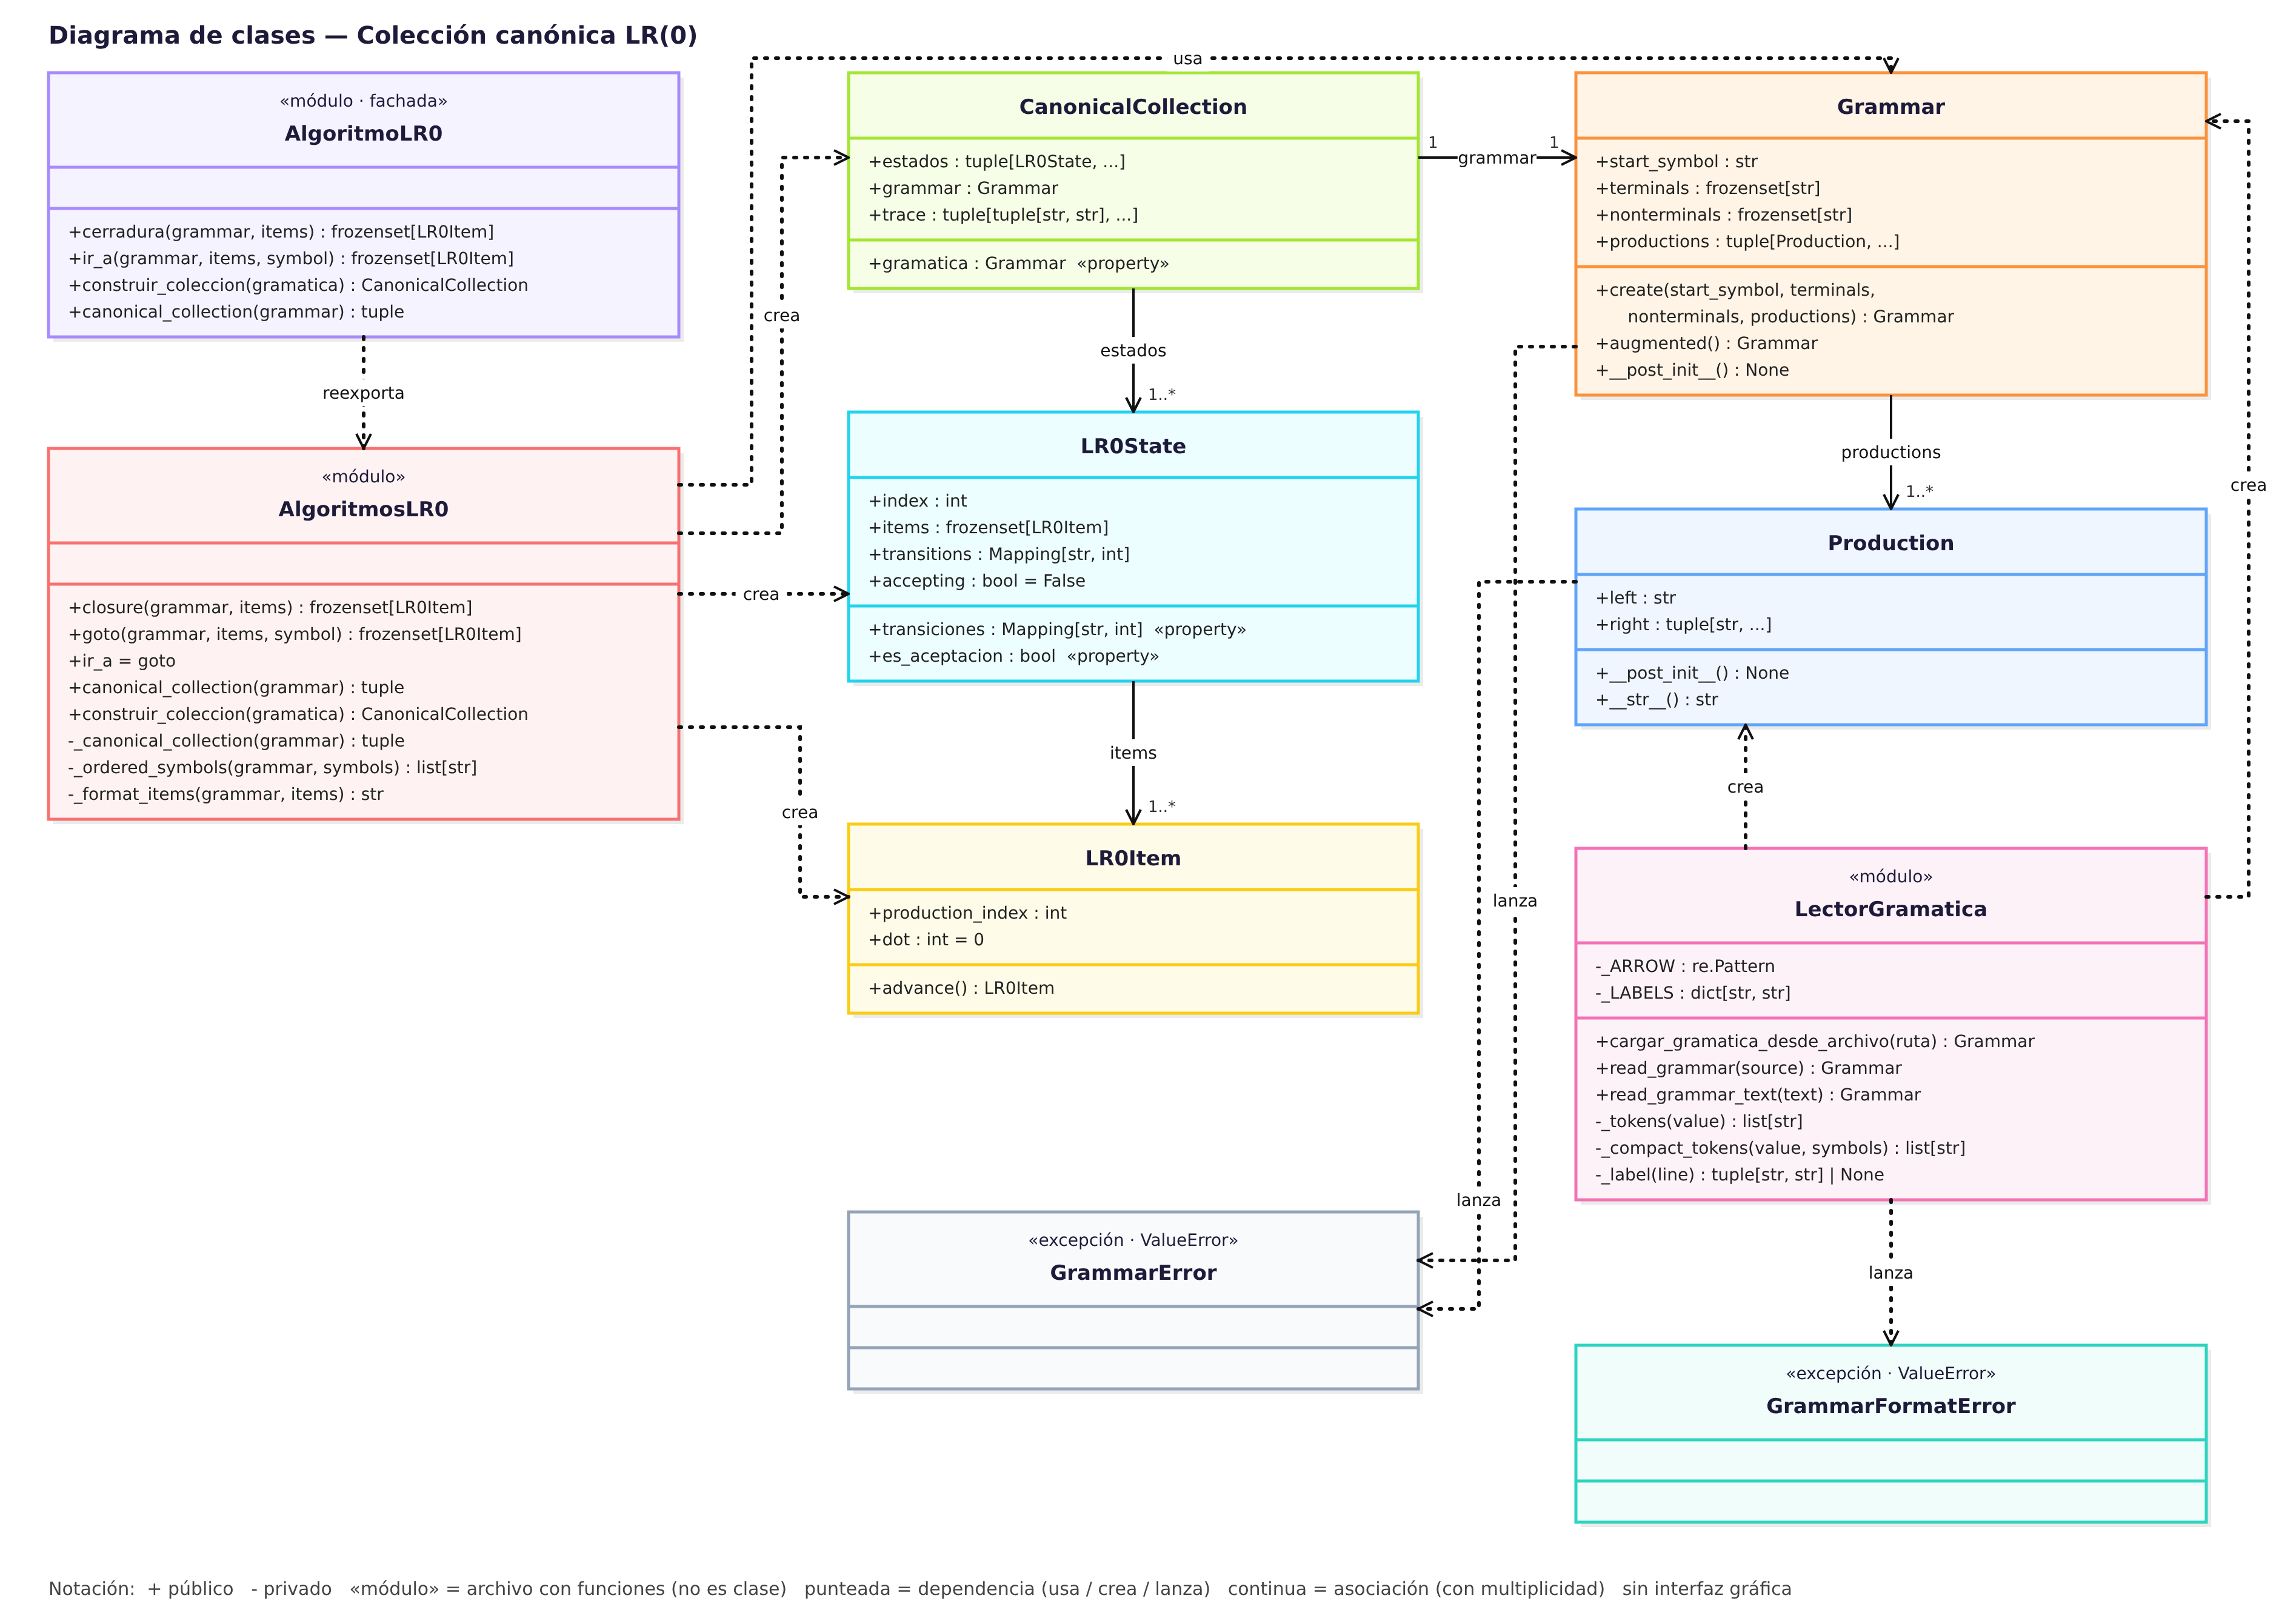
\includegraphics[width=\linewidth, keepaspectratio]{imagenes/diagrama_clases_lr0.png}
  \vspace{0.4cm}
  \caption{Diagrama de clases del sistema Colección Canónica LR(0).}
\end{figure}
\vspace*{\fill}
\end{landscape}
